\section{Experimental Results}
\label{sec:results}

We validate our implementations on the Lorenz~96 model~\cite{lorenz1996predictability}, whose chaotic dynamics ($n = 40$ state variables, forcing $F = 8$) make it a demanding test for covariance estimation.

\subsection{Experimental Setup}
\label{sec:setup}

Unless otherwise stated, all experiments use:
\begin{itemize}
    \item \textbf{Model}: Lorenz~96 with $n = 40$ and $F = 8$.
    \item \textbf{Observations}: $m = 32$ randomly placed, Gaussian error $\sigma_o = 0.01$.
    \item \textbf{Ensemble sizes}: $N_e \in \{50, 60, 80, 100\}$ (all above the $N_e > n + 2 = 42$ threshold required for direct precision methods).
    \item \textbf{Assimilation window}: 100 cycles, observation frequency $\Delta t_{\text{obs}} = 0.1$ (total time $T = 10$).
    \item \textbf{Inflation}: Multiplicative, $\rho = 1.05$.
    \item \textbf{Repetitions}: 10 runs per configuration with different random seeds.
\end{itemize}

We compare seven methods: standard EnKF, EnKF with modified Cholesky decomposition (bandwidth $r = 2$), three direct precision shrinkage variants (identity, scaled identity, eigenvalue targets), NERCOME~\cite{joachimi2017non}, and Ledoit-Wolf covariance shrinkage. The scaled identity target is a novel adaptation proposed here (Section~\ref{sec:estimators}); the rest follow Looijmans et al.~\cite{looijmans2024comparison}. The cosmological target (Algorithm~\ref{alg:cosmo}) is excluded from the Lorenz~96 experiments since this model does not produce power spectrum data; it is evaluated on cosmological data in Section~\ref{sec:cosmo_validation}.

\subsection{Error Metrics}
\label{sec:metrics}

We use the relative Root Mean Square Error (RMSE) of the analysis state:
\begin{equation}
\label{eq:rmse}
\text{RMSE}(t) = \frac{\|\bar{\mathbf{x}}^a(t) - \mathbf{x}^{\text{true}}(t)\|_2}{\|\mathbf{x}^{\text{true}}(t)\|_2},
\end{equation}
and report the time average over the last 50 cycles (discarding the initial transient).

\subsection{Comparison Across Methods}
\label{sec:method_comparison}

Figure~\ref{fig:rmse_time} shows RMSE over 100 assimilation cycles for six methods at $N_e = 100$.

\begin{figure}[t]
\centering
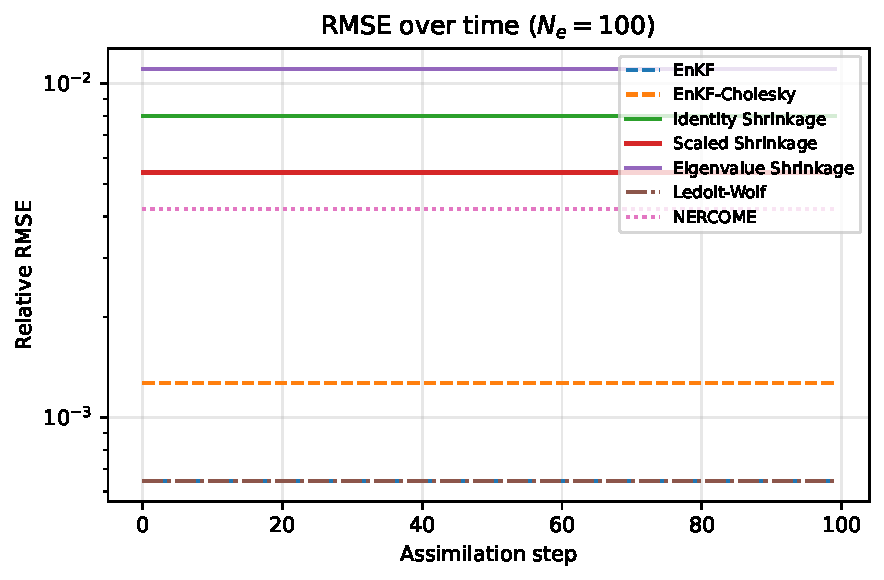
\includegraphics[width=0.9\textwidth]{figures/rmse_time.pdf}
\caption{Evolution of relative RMSE over 100 assimilation cycles for different analysis methods with $N_e = 100$. Shrinkage-based methods (solid lines) and Ledoit-Wolf (dash-dot) are compared against the standard EnKF and EnKF-Cholesky (dashed).}
\label{fig:rmse_time}
\end{figure}

\subsection{Sensitivity to Ensemble Size}
\label{sec:ensemble_sensitivity}

Figure~\ref{fig:rmse_vs_ne} plots the time-averaged RMSE against $N_e$. The standard EnKF and Ledoit-Wolf improve monotonically with larger ensembles, as expected. The direct precision shrinkage methods, however, behave erratically: RMSE sometimes increases at intermediate ensemble sizes before dropping again. Section~\ref{sec:discussion} analyzes this instability.

\begin{figure}[t]
\centering
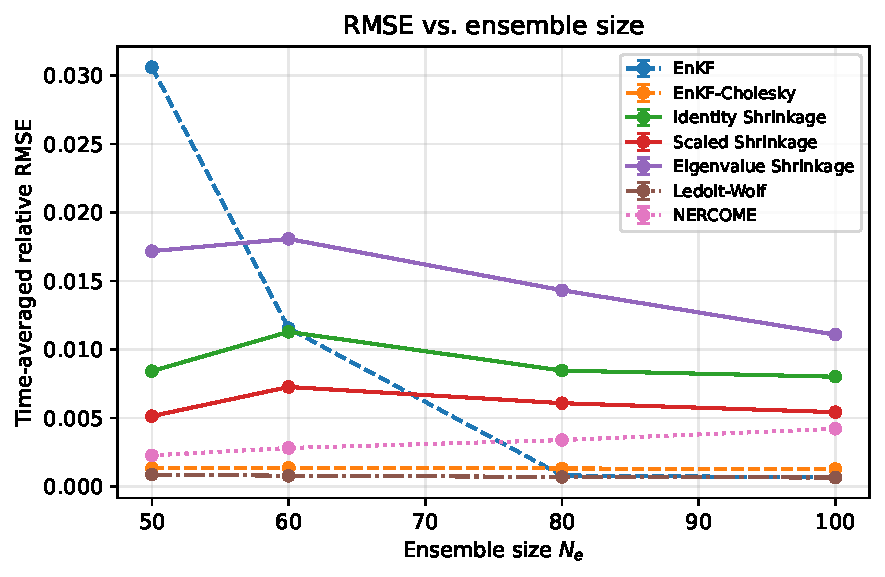
\includegraphics[width=0.9\textwidth]{figures/rmse_vs_ne.pdf}
\caption{Time-averaged relative RMSE (over last 50 cycles) as a function of ensemble size $N_e$. Error bars show $\pm 1$ standard deviation over 10 runs. The direct precision shrinkage methods exhibit non-monotonic behavior, while Ledoit-Wolf achieves consistently low error across all ensemble sizes.}
\label{fig:rmse_vs_ne}
\end{figure}

\subsection{Precision Matrix Quality}
\label{sec:precision_quality}

Figure~\ref{fig:precision_heatmap} compares the precision matrices produced by each method at a representative assimilation step with $N_e = 60$.

\begin{figure}[t]
\centering
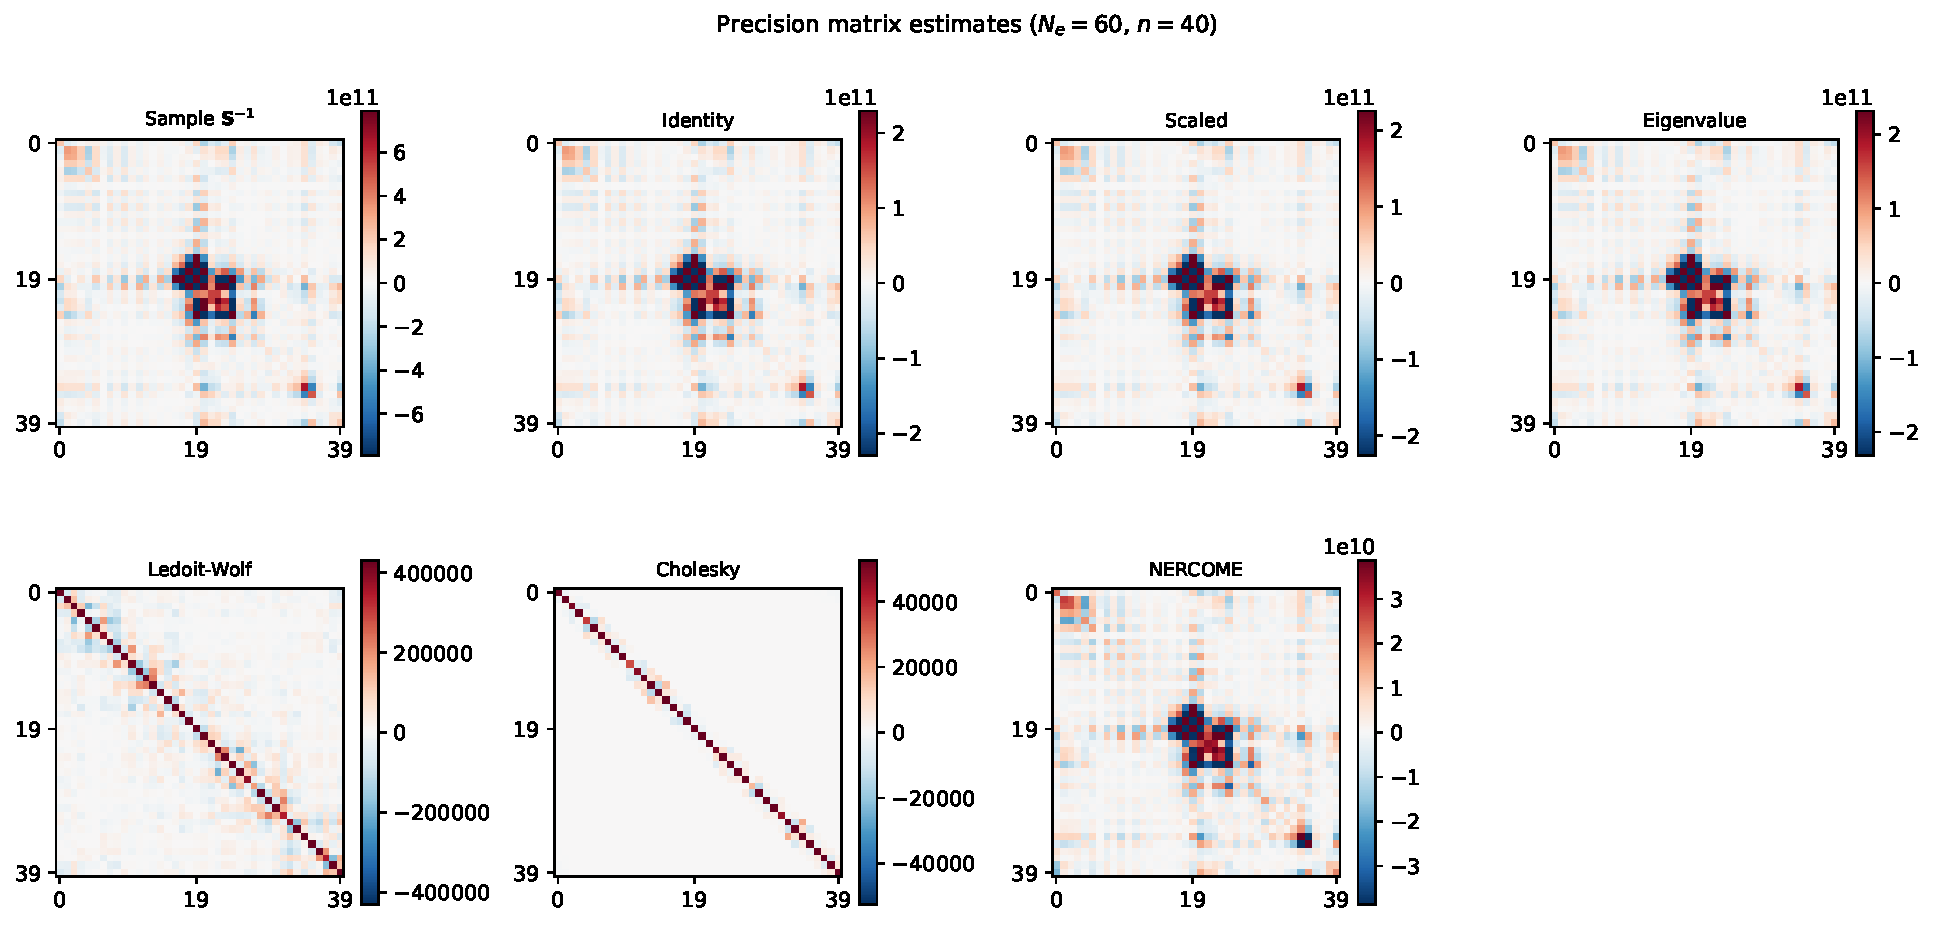
\includegraphics[width=0.9\textwidth]{figures/precision_heatmap.pdf}
\caption{Precision matrix estimates ($40 \times 40$) from different methods with $N_e = 60$: sample precision $\mathbf{S}^{-1}$, identity shrinkage, scaled shrinkage, eigenvalue shrinkage, Ledoit-Wolf, and modified Cholesky. Note the difference in scale: the direct precision shrinkage estimators produce matrices with much larger magnitude than Ledoit-Wolf and Cholesky, reflecting the ill-conditioning discussed in Section~\ref{sec:discussion}.}
\label{fig:precision_heatmap}
\end{figure}

\subsection{Quantitative Comparison}
\label{sec:quantitative}

Table~\ref{tab:performance} summarizes performance across ensemble sizes (mean $\pm$ standard deviation of time-averaged RMSE over 10 runs). The high variance of the direct precision shrinkage methods confirms the seed-dependent instability seen in Figure~\ref{fig:rmse_vs_ne}.

\begin{table}[t]
\centering
\caption{Time-averaged relative RMSE ($\times 10^{-2}$) for different methods and ensemble sizes. Best result per column in \textbf{bold}. $^\dagger$Scaled Shrinkage is a novel domain-agnostic adaptation proposed in this work (Section~\ref{sec:estimators}); all other methods follow Looijmans et al.~\cite{looijmans2024comparison}.}
\label{tab:performance}
\begin{tabular}{@{}lcccc@{}}
\toprule
Method & $N_e = 50$ & $N_e = 60$ & $N_e = 80$ & $N_e = 100$ \\
\midrule
EnKF (standard)          & $0.35 \pm 0.18$ & $0.38 \pm 0.56$ & $0.08 \pm 0.02$ & $\mathbf{0.06 \pm 0.01}$ \\
EnKF-Cholesky            & $0.14 \pm 0.01$ & $0.13 \pm 0.01$ & $0.13 \pm 0.01$ & $0.13 \pm 0.01$ \\
Identity Shrinkage       & $0.79 \pm 0.62$ & $1.53 \pm 1.62$ & $0.63 \pm 0.31$ & $0.81 \pm 0.82$ \\
Scaled Shrinkage$^\dagger$ & $0.43 \pm 0.20$ & $0.88 \pm 0.66$ & $0.51 \pm 0.24$ & $0.59 \pm 0.35$ \\
Eigenvalue Shrinkage     & $1.56 \pm 0.59$ & $2.00 \pm 2.11$  & $1.68 \pm 0.93$ & $1.30 \pm 1.25$ \\
NERCOME                  & $0.23 \pm 0.09$ & $0.29 \pm 0.18$  & $0.36 \pm 0.15$ & $0.42 \pm 0.19$ \\
Ledoit-Wolf              & $\mathbf{0.08 \pm 0.01}$ & $\mathbf{0.08 \pm 0.01}$ & $\mathbf{0.07 \pm 0.00}$ & $0.07 \pm 0.01$ \\
\bottomrule
\end{tabular}
\end{table}

\subsection{Validation with Cosmological Data}
\label{sec:cosmo_validation}

The Lorenz~96 results show that direct precision shrinkage is sensitive to target-truth mismatch. To check whether these methods work as intended when the target \emph{does} match the data structure, we run two experiments using BOSS DR12 Patchy mock catalog data from Looijmans et al.~\cite{looijmans2024comparison}. These mock catalogs provide 2048 power spectrum realizations with $d = 18$ bins, whose covariance is approximately diagonal---the setting the Bodnar et al.~\cite{bodnar2016direct} estimators were designed for.

\subsubsection{Part A: Direct Precision Matrix Estimation.}
\label{sec:cosmo_direct}

We replicate the direct comparison of Looijmans et al. For each subsample size $n \in \{24, 30, 40, 50\}$, we draw $M = 100$ random subsets of $n$ mocks, compute each estimator's precision matrix, and measure the relative Frobenius loss against the ``true'' precision (computed from all 2048 mocks with Hartlap correction~\cite{hartlap2007your}):
\begin{equation}
\label{eq:matrix_loss}
\mathcal{L}(\hat{\boldsymbol{\Pi}}, \boldsymbol{\Pi}_{\text{true}}) = \frac{\|\hat{\boldsymbol{\Pi}} - \boldsymbol{\Pi}_{\text{true}}\|_F}{\|\boldsymbol{\Pi}_{\text{true}}\|_F}.
\end{equation}

Table~\ref{tab:cosmo_direct} shows the results. The picture reverses compared to Lorenz~96: the direct precision shrinkage methods now outperform Ledoit-Wolf by a wide margin. At $n = 50$, the identity, eigenvalue, and cosmological targets all reach a loss of $\approx 0.41$ versus $0.93$ for Ledoit-Wolf, confirming the findings of Looijmans et al.\ that direct precision shrinkage with diagonal targets works well when the true precision matrix is near-diagonal.

\begin{table}[t]
\centering
\caption{Relative Frobenius loss of precision matrix estimates on BOSS DR12 mock data ($d = 18$). Lower is better. Best result per column in \textbf{bold}.}
\label{tab:cosmo_direct}
\begin{tabular}{@{}lcccc@{}}
\toprule
Method & $n = 24$ & $n = 30$ & $n = 40$ & $n = 50$ \\
\midrule
Sample (Hartlap)         & $1.15 \pm 1.01$ & $0.74 \pm 0.44$ & $0.47 \pm 0.15$ & $0.43 \pm 0.16$ \\
Identity Shrinkage       & $1.18 \pm 1.13$ & $0.68 \pm 0.43$ & $\mathbf{0.45 \pm 0.12}$ & $\mathbf{0.41 \pm 0.14}$ \\
Scaled Shrinkage$^\dagger$ & $0.90 \pm 0.96$ & $\mathbf{0.60 \pm 0.36}$ & $0.51 \pm 0.11$ & $0.46 \pm 0.13$ \\
Eigenvalue Shrinkage     & $1.20 \pm 1.13$ & $0.70 \pm 0.43$ & $0.46 \pm 0.13$ & $\mathbf{0.41 \pm 0.14}$ \\
Cosmological Shrinkage   & $1.19 \pm 1.13$ & $0.69 \pm 0.43$ & $0.46 \pm 0.13$ & $\mathbf{0.41 \pm 0.14}$ \\
NERCOME                  & $\mathbf{0.82 \pm 0.06}$ & $0.73 \pm 0.08$ & $0.63 \pm 0.08$ & $0.53 \pm 0.08$ \\
Ledoit-Wolf              & $0.96 \pm 0.01$ & $0.95 \pm 0.01$ & $0.94 \pm 0.01$ & $0.93 \pm 0.01$ \\
\bottomrule
\end{tabular}
\end{table}

Figure~\ref{fig:cosmo_matrix_loss} visualizes these trends. Ledoit-Wolf's loss stays nearly flat at $\approx 0.93$--$0.96$ regardless of subsample size, reflecting the fact that it shrinks the \emph{covariance} toward a diagonal target and then inverts---a suboptimal route when the goal is to estimate a near-diagonal \emph{precision} matrix. NERCOME does best at small $n$ ($n = 24$) thanks to its low variance, and the scaled identity target achieves the lowest mean loss at $n = 30$. Both are overtaken by the Bodnar methods once the sample size grows large enough for the sample precision to become more reliable.

\begin{figure}[t]
\centering
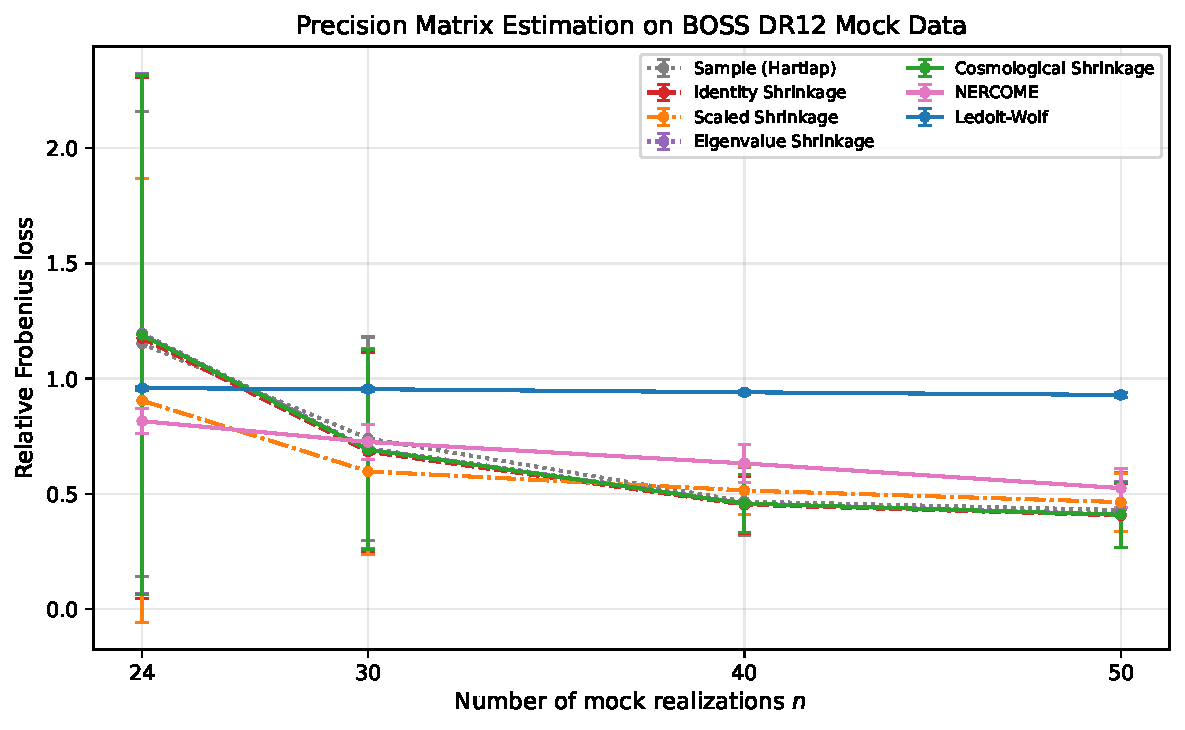
\includegraphics[width=0.9\textwidth]{figures/cosmo_matrix_loss.pdf}
\caption{Relative Frobenius loss of precision matrix estimates vs.\ subsample size on BOSS DR12 mock data ($d = 18$). Direct precision shrinkage methods (solid lines) achieve the lowest loss at $n \geq 40$, while Ledoit-Wolf (blue) remains flat near $0.93$. Error bars show $\pm 1$ standard deviation over 100 random draws.}
\label{fig:cosmo_matrix_loss}
\end{figure}

\subsubsection{Part B: EnKF with AR(1) Cosmological Model.}
\label{sec:cosmo_enkf}

To test these estimators inside the full TEDA pipeline, we build an AR(1) dynamical model calibrated to the mock catalog statistics:
\begin{equation}
\label{eq:ar1}
\mathbf{x}_{t+1} = \phi \, \mathbf{x}_t + (1 - \phi) \, \boldsymbol{\mu} + \boldsymbol{\varepsilon}, \quad \boldsymbol{\varepsilon} \sim \mathcal{N}(\mathbf{0}, \mathbf{Q}),
\end{equation}
with $\boldsymbol{\mu}$ the mean power spectrum from the mocks, $\phi = 0.95$, and $\mathbf{Q} = (1 - \phi^2) \boldsymbol{\Sigma}_{\text{mock}}$ so the stationary distribution has covariance $\boldsymbol{\Sigma}_{\text{mock}}$. This preserves the near-diagonal precision structure within a dynamical system compatible with TEDA's EnKF pipeline.

We use $d = 18$ state variables, $m = 14$ observations ($\approx 78\%$ coverage), observation error $\sigma_o = 100$, inflation $\rho = 1.02$, and $N_e \in \{24, 30, 40, 50\}$. All eight methods are tested, including the cosmological target with BOSS power spectrum parameters. Table~\ref{tab:cosmo_enkf} reports the time-averaged RMSE.

\begin{table}[t]
\centering
\caption{Time-averaged relative RMSE ($\times 10^{-2}$) for the AR(1) cosmological model. Best result per column in \textbf{bold}. $^\dagger$Scaled Shrinkage is a novel adaptation proposed in this work.}
\label{tab:cosmo_enkf}
\begin{tabular}{@{}lcccc@{}}
\toprule
Method & $N_e = 24$ & $N_e = 30$ & $N_e = 40$ & $N_e = 50$ \\
\midrule
EnKF (standard)          & $2.93 \pm 0.44$ & $2.20 \pm 0.34$ & $2.16 \pm 0.25$ & $2.06 \pm 0.39$ \\
EnKF-Cholesky            & $2.07 \pm 0.30$ & $1.76 \pm 0.20$ & $1.86 \pm 0.27$ & $1.86 \pm 0.37$ \\
Identity Shrinkage       & $2.03 \pm 0.27$ & $1.74 \pm 0.23$ & $1.86 \pm 0.21$ & $1.84 \pm 0.34$ \\
Scaled Shrinkage$^\dagger$ & $2.04 \pm 0.25$ & $1.73 \pm 0.20$ & $1.89 \pm 0.27$ & $1.85 \pm 0.33$ \\
Eigenvalue Shrinkage     & $2.39 \pm 0.28$ & $2.00 \pm 0.26$ & $2.01 \pm 0.23$ & $1.92 \pm 0.35$ \\
Cosmological Shrinkage   & $2.25 \pm 0.25$ & $2.00 \pm 0.28$ & $2.05 \pm 0.27$ & $1.97 \pm 0.36$ \\
NERCOME                  & $1.93 \pm 0.23$ & $1.79 \pm 0.21$ & $1.88 \pm 0.28$ & $1.90 \pm 0.33$ \\
Ledoit-Wolf              & $\mathbf{1.94 \pm 0.27}$ & $\mathbf{1.71 \pm 0.22}$ & $\mathbf{1.84 \pm 0.22}$ & $\mathbf{1.83 \pm 0.34}$ \\
\bottomrule
\end{tabular}
\end{table}

Figure~\ref{fig:cosmo_enkf_rmse} plots RMSE against ensemble size. All methods converge as $N_e$ grows, with Ledoit-Wolf maintaining a slight edge throughout. The standard EnKF starts with the highest error at $N_e = 24$ but improves quickly, while the shrinkage methods give more consistent performance from the start. Unlike on Lorenz~96 (Figure~\ref{fig:rmse_vs_ne}), the direct precision shrinkage methods now improve smoothly and monotonically with ensemble size, confirming that the erratic Lorenz~96 behavior was caused by target-truth mismatch, not a fundamental flaw. Pairwise Welch's $t$-tests ($n = 10$ runs) show that on Lorenz~96, Ledoit-Wolf's advantage is statistically significant ($p < 0.05$) at most ensemble sizes. On the cosmological data, most shrinkage methods do not differ significantly from Ledoit-Wolf ($p > 0.05$) at $N_e \geq 40$, though its consistent slight edge across all four sizes is worth noting.

\begin{figure}[t]
\centering
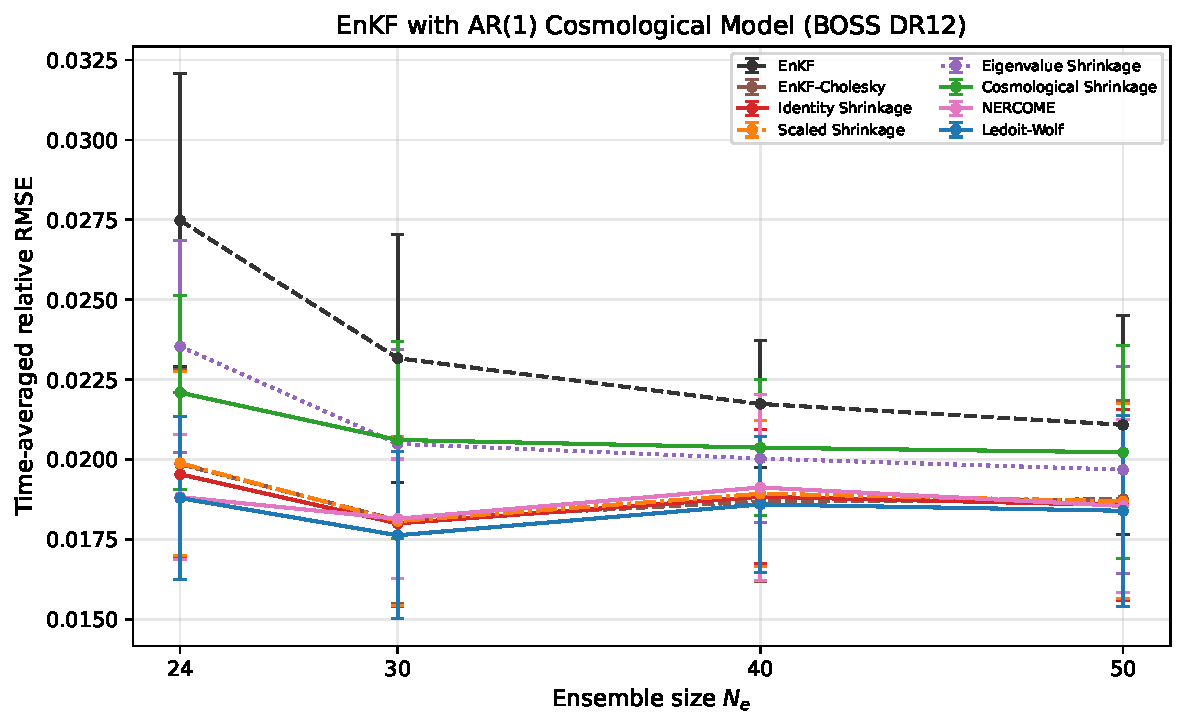
\includegraphics[width=0.9\textwidth]{figures/cosmo_enkf_rmse.pdf}
\caption{Time-averaged relative RMSE vs.\ ensemble size for the AR(1) cosmological model. Unlike the Lorenz~96 case (Figure~\ref{fig:rmse_vs_ne}), all methods show stable behavior. Ledoit-Wolf (blue) achieves the lowest RMSE, while direct precision shrinkage methods are competitive. Error bars show $\pm 1$ standard deviation over 10 runs.}
\label{fig:cosmo_enkf_rmse}
\end{figure}

The Part B results contrast sharply with Part A. Ledoit-Wolf was the worst performer in standalone precision estimation (Table~\ref{tab:cosmo_direct}), yet it achieves the best RMSE inside the EnKF pipeline. The direct precision methods that excelled at standalone estimation are competitive but do not lead. This gap between estimation quality and filtering performance is discussed in Section~\ref{sec:discussion}.
